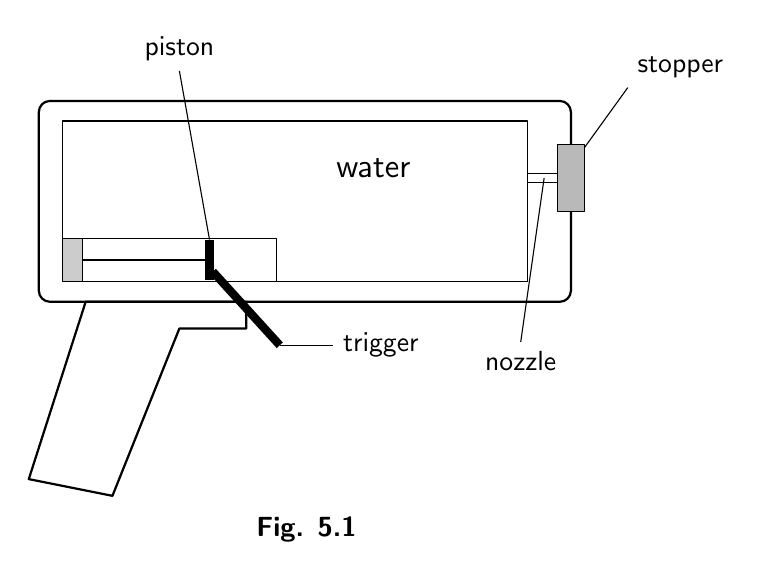
\begin{tikzpicture}[scale=0.85, font=\sffamily, line join=round]
  % handle
  \draw[thick, fill=white] (0.7,2.0)--(3.1,2.0)--(3.1,1.6)--(2.1,1.6)--(1.1,-0.9)--(-0.15,-0.65)--cycle;
  % body
  \draw[thick, rounded corners=4pt] (0,2) rectangle (7.95,5);
  % water reservoir
  \dotregion{0.35}{2.3}{7.3}{4.7}
  \draw (0.35,2.3) rectangle (7.3,4.7);
  \node[fill=white, inner sep=2pt, font=\sffamily\large] at (5,4) {water};
  % cylinder, piston, rod and trigger
  \draw[fill=white] (0.35,2.3) rectangle (3.55,2.95);
  \draw[fill=gray!40] (0.35,2.3) rectangle (0.65,2.95);
  \draw[thick] (0.65,2.62)--(2.55,2.62);
  \draw[line width=3pt] (2.55,2.32)--(2.55,2.93);
  \draw[line width=3pt] (2.6,2.45)--(3.6,1.35);
  % nozzle and stopper
  \draw[fill=white] (7.3,3.78) rectangle (7.75,3.92);
  \draw[fill=gray!55] (7.75,3.35) rectangle (8.15,4.35);
  % labels
  \draw (2.55,2.93)--(2.1,5.45) node[above] {piston};
  \draw (3.6,1.35)--(4.4,1.35) node[right] {trigger};
  \draw (7.55,3.85)--(7.2,1.4) node[below] {nozzle};
  \draw (8.15,4.3)--(8.8,5.2) node[above right] {stopper};
  \node[font=\sffamily\bfseries] at (4,-1.4) {Fig. 5.1};
\end{tikzpicture}
